\documentclass[]{IEEEtran}
\usepackage[utf8]{inputenc}
\usepackage[english]{babel}

\title{Scooter Trajectories Clustering\\
	{\large University of Verona\\Computer Engineering for Robotics and Smart Industry\\Machine Learning and Deep Learning\\2020/2021\\}}
\author{Mirco De Marchi - VR445319}

%\usepackage{algorithm,algorithmic}

\usepackage{hyperref}
\hypersetup{
    linktoc=all
}

\usepackage{graphicx}
\graphicspath{ {../image/} }

\usepackage{listings}

% Table environment
\usepackage{tabularx}
\renewcommand{\arraystretch}{1.2}
\usepackage{float}
\restylefloat{table}

\usepackage{amsmath}

\usepackage{tikz}
\usetikzlibrary{positioning,shapes,shadows,arrows}

\usepackage{multicol}
%\setlength{\multicolsep}{6.0pt plus 2.0pt minus 1.5pt}% 50% of original values
\setlength\multicolsep{0pt}

\begin{document}
\maketitle

% ABSTRACT
\begin{abstract}
	The aim of this report is to present the main unsupervised learning techniques used for scooter trajectories clustering. The dataset that I used contains a big amount of positions taken in rentals that run through some cities in Italy. The objective is to find recurrent places crossed by the trajectories. This report presents some analysis on the positions and an implementation of heuristics that manage data in a systematic way: \textit{timedelta heuristic}, \textit{spreaddelta heuristic}, \textit{edgedelta heuristic} and \textit{coorddelta heuristic}. Then I performed the most traditional machine learning clustering techniques on the generated dataset: \textit{K-Means}, \textit{Mean Shift}, \textit{Gaussian Mixture}, \textit{Full Hierarchical Agglomerative}, \textit{Ward Hierarchical Agglomerative}. All the features are extracted with \textit{Principal Component Analysis (PCA)} with an improvement that select the components to focus on and have been integrated with the informations obtained from the heuristic procedures in order to optimize feature extraction.
\end{abstract}

% INTRODUZIONE
\section{Motivation}
Motion trajectories are really difficult to analyse and handle because of the amount of data. There could be errors in position tracking, due to localization issues, and usually data are not organized as you expect. Consequently trajectories are difficult to represent, filter and manage in relation with themselves or other informations. First of all, trajectories clustering is a challenge for its intrinsic difficulty in being treated and today is an ambitious topic in data science research. Moreover, trajectory clustering can help for several applications:
\begin{itemize}
	\item Monitoring: understand main points of interest and common places visited by tourists;
	\item Forecasting: prediction of possible destinations starting from the current position and previous ones; 
	\item Viability: traffic monitoring and kind of user's activity extracting semantic concepts from trajectories;
	\item Smart city: data support to city plan and smart transportation management;
	\item Security: trajectories which are significantly different from others in terms of some similarity metric may be viewed as outliers;
	\item Video analysis: movement pattern analysis from video (after extracting trajectories from video data);
\end{itemize}


% BACKGROUND
\section{State of art}
In \cite{AIReview} book there are some techniques widely used for clustering of moving object. Some methodology are pretty new but there are also some historical algorithm that provides good results: 
\begin{itemize}
	\item K-Means: 
	\item CURE:
	\item Birch:
	\item DBSCAN:
	\item Optics:
	\item Sting:
	\item Cosweb
\end{itemize}

% METODOLOGIA
\section{Objectives}
The objectives of this project is grouping trajectories in order to find common locations crossed by people that rent a scooter to visit a city in Italy. The model built has to be able to distinguish for example the positions related to a trajectory that takes from the train station to the city centre, the ones that move in the city centre, the ones that run through the periphery and so on. 

In particular the steps that involves the project are:
\begin{enumerate}
	\item Dataset filtering and merging in order to build a dataset tidier and semantically correct;
	\item Analyse features and represent the trajectories in line plots;
	\item Group the positions for each rental and sort them through the timestamp;
	\item Apply heuristic techniques on features;
	\item Apply unsupervised learning techniques on features (as K-Means, Mean Shift...);  
	\item Study the results and evaluate the goodness of clustering;
\end{enumerate}

% METHODOLOGY
\section{Methodology}
The original dataset is composed by 4 tables in CSV fomat: \textit{pos.csv}, \textit{rental.csv}, \textit{user.csv}, \textit{device.csv}. This dataset is a subset of an another dataset with some sensitive data dropped (as user name or email) and positions manumit in order to protect proprietary data. Although the data are only a subset of the proprietary data, the amount positions is really huge and it weighs about 2GB. 

The \textit{pos.csv} table contains all the positions, characterized by latitude, longitude, speed, timestamp and a device id used to join with \textit{device.csv} table. The \textit{device.csv} and \textit{user.csv} tables contain the kilometers traveled respectively by a scooter and by a user. At last, the \textit{rental.csv} table contains the longitude and latitude positions of rental starting and ending points with related timestamp, and all the ids used to join the other tables with this one. 

The first thing that I have noticed is that the dataset is not built very well, because the informations referenced are not semantically correct. In fact, I would have the positions in relation with the rental and not with the device, therefore I tried to join the tables and I noticed that each rental is referenced by an unique device id. It means that there not exist multiple device used in different rental, but the device table is used only to take the positions in relation with rentals. Moreover I noticed that not all positions data have a matched rental, and not all rentals have some matched positions. This is caused by the subset extraction and the previous operation performed to protect sensitive informations. It means that the dataset can be filtered and reduced in size.

As result of this first analysis I implemented an algorithm that filters and joins the table in a single one, in order to have simpler data to handle. This operation was really tricky because the total amount of data is huge and I had to use optimized functions based on database join algorithms and chunks management to be able to handle these data in shot time. At last, the resulting table has been sorted for rental id, position id and timestamp, in order to have everything ready to perform plot representation and some feature analysis.

After that I performed some analysis on the features. I studied their distribution and I started to think how could be possible to group or divide positions. In particular I learnt that two trajectories can be similar in shape and can be divided in time. It means that a sequence of positions, a trajectory, can be similar to another one, evaluating his shape appearance and location in the geographical map, and therefore his sequence of latitude and longitude. On the other hand a trajectory can be different to another one if there is a temporal space between each other. The starting assumption of this analysis is that all positions belong to a rental, it means that starting from how data are constructed, I assume that a trajectory is the sequence of positions sorted in time that belong to the same rental. As result I implemented 3 different clustering heuristics performed in a systematic and statistical way on the entire sequence of positions:
\begin{itemize}
	\item \textbf{timedelta heuristic}: considers that a trajectory of a rental can be divided in a sequence of trajectories if the time gap between a position and previous one exceeds a \textit{timedelta} value. First of all I calculated the time gaps for each set of positions grouping in rental: 
	\begin{align}
		TIMEGAPS = \{p.time - p[-1].time \mid \forall p \in POS \}
	\end{align}
	where \verb|p[-1]| is the previous position and the field \verb|.time| is the related timestamp. The \textit{timedelta} value can be assigned by a user that runs the heuristic process or can be automatically calculated. To calculate automatically the timedelta value I plotted the timegaps distribution, I noticed that the curve is unimodal and I assumed to approximate it as a normal distribution. Therefore I assigned the timegaps standard deviation to my timedelta in order to exploit the statistical empirical rule and cover a percentage of timegaps distribution. In this case I take all the left tail of the distribution and the $43\%$ of the right one, and that ones that remains outside are the positions candidates that divide a trajectory from another one. This operation has been performed for each rental positions in order to obtain a set of sub-trajectories of rental trajectory.
	\item \textbf{spreaddelta heuristic}: considers that a trajectory of a rental can be considered similar to another one if they spread the same area. I calculate the spread area for each rental trajectory in the following way: 
	\begin{align}
		SPREADS = \{max(t) - min(t) \mid \forall t \in TRAJ \}
	\end{align}
	where \verb|max(t)| and \verb|min(t)| calculate respectively the maximum and the minimum latitude and longitude of a set of positions, and \verb|TRAJ| is the set of trajectories that can be grouped for each rental, but even for timedelta heuristic previously calculated in order to consider the time gaps division of trajectory and not only the rental division. Also in this case the result of spread distribution is a unimodal curve that can be approximated in a normal distribution and I have again exploited the empirical rule to compute the trajectories similar for spread. I assigned $std(SPREADS) / 4$ to the spreaddelta if you want to automatically calculate it, otherwise of course you can choose the value of spreaddelta. If automatically calculated, the spreaddelta will cover the spread distribution of about $20\%$. This operation will be repeated as long as all the positions has spread id assigned, and when a position is assigned it is discarded from the distribution calculus. 
	\item \textbf{edgedelta heuristic}: acts as the spreaddelta heuristic, but it consider the edge of a trajectory, or rather the first position and the last position of the trajectory. The main problem here is that the distribution of edge positions has 2 centres or, in other words, it is bimodal. In fact the dataset positions involves mainly in 2 different cities of Italy, and this translates in a bimodal distribution of the positions. In this case I can't use the distribution mean or the standard deviation because they should result wrong, but I have to approximate these values. To resolve this issue I applied for simplicity only 1 iteration of Mean Shift starting from a random position in order to get closer to a centre of the distribution (one of the two indifferently) and to obtain a spread subset more significant to calculate the deviation standard and use it as edgedelta. In particular the value assign to edgedelta is $std(meanshift(EDGES, iter=1)) * 2$ and obtain the $95\%$ of the subset of edges found by meanshift. The set of edges is calculated in the following way: 
	\begin{align}
		EDGES = \{concat(p[0], p[-1]) \mid \forall t \in TRAJ \}
	\end{align}
 	\item \textbf{coorddelta heuristic}: it is a combination spread and edge heuristics and combine the main advantages of each other. To guarantee the convergence of this algorithm edge heuristic and spread heuristic have to manage the same subset of trajectory. Therefore first it is applied edge heuristic to find a subset of trajectories near a distribution centre and then both heuristics, edge and spread, are applied to same subset.
\end{itemize}

After the implementation of these heuristic techniques, I started to prepare the features to be processed by clustering algorithms. In particular I decided to perform Standardization, Normalization and than Principal Component Analysis (PCA) on features. The component extracted by PCA can be dediced in 3 different ways:
\begin{enumerate}
	\item By a number of component decided a priori;
	\item By the cumulative variance calculated by PCA over the number of features, considering to cover almost an $80\%$ of variance;
	\item Constructing a list of features subset and performing PCA to produce 1 component for each features subset. The result will be a concatenation of columns produced by PCA for different subset of features.
\end{enumerate}

As feature extraction, I considered that the work done for the heuristic algorithm could return useful for clustering algorithms. In particular $TIMEGAPS$, $SPREADS$ and $EDGES$ sets can be used as new features of my data. Therefore I integrate my data features with the ones extracted from the heuristic and I used it to be processed with Standardization, Normalization, PCA and than clustering algorithms.

The clustering algorithms that I used are the following: 
\begin{itemize}
	\item \textbf{K-Means}:
	\item \textbf{Mean Shift}:
	\item \textbf{Gaussian Mixture}:
	\item \textbf{Full Hierarchy}:
	\item \textbf{Ward Hierarchy}: 
\end{itemize}

% RESULTS
\section{Results}
The best way to show the clustering results is plotting the trajectory with different colours in relation to the cluster which it belongs. In addiction, for clustering algorithms, I used a method of interpretation and validation of consistency within clusters of data, called \textit{Silhouette}. 

\textit{Silhouette} clustering validation technique measures how similar an object is to its own cluster compared to other clusters. The silhouette ranges from -1 to +1, where a high value indicates that the object is well matched to its own cluster and poorly matched to neighbouring clusters.

The results of heuristic analysis are the following: 
\begin{itemize}
	\item \textit{timedelta heuristic}: is the heuristic that perform the best result. In figure \ref{fig:timedelta-result} you can see some rentals with their positions divided in subgroups of trajectories. That sub trajectories are built considering only the time gaps between the positions, no latitude or longitude has been used to produce this result. This result shows how the time sequences could be really useful to produce a good trajectory partition. Moreover, in figure \ref{fig:timedelta-lineplot}, there is the \textit{timedelta heuristic} representation in the entire city.
	
	\begin{figure}[bt]
		\centering
		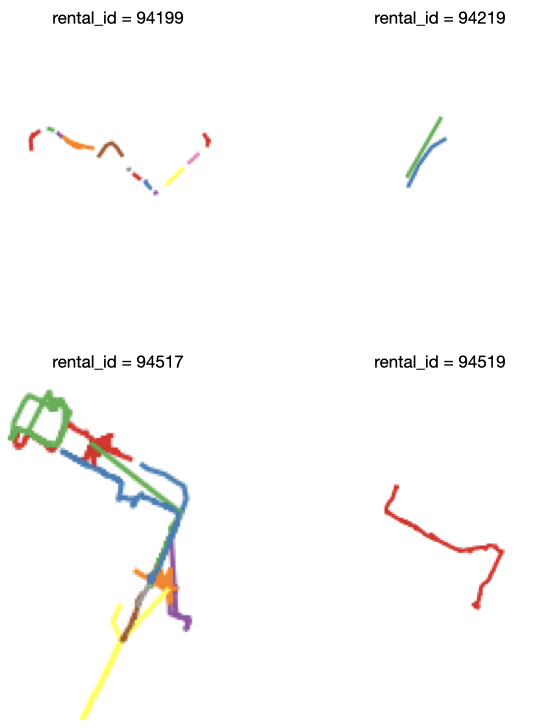
\includegraphics[width=\columnwidth]{timedelta-result}
		\caption{Timedelta heuristic line plot in details}
		\label{fig:timedelta-result}
	\end{figure}

	\begin{figure}[bt]
		\centering
		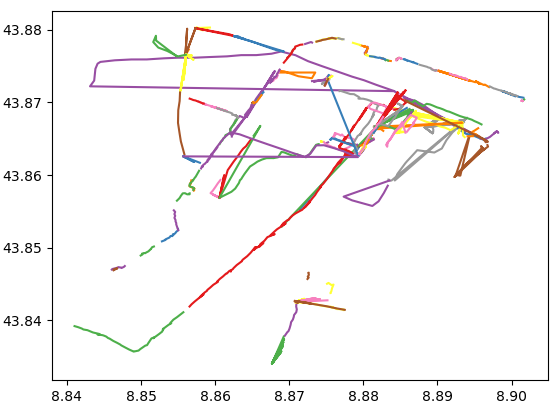
\includegraphics[width=\columnwidth]{timedelta-lineplot}
		\caption{Timedelta heuristic line plot in the entire city}
		\label{fig:timedelta-lineplot}
	\end{figure}

	\item \textit{spreddelta heuristic}: in figure \ref{fig:spreaddelta-result} you can see how the trajectories are clusterized in 3 main groups: wide area trajectories (green), medium area trajectories (blue) and small area trajectories (red). The trajectories showed in figure are grouped starting from the \textit{timedelta} division performed before. 
	
	\begin{figure}[bt]
		\centering
		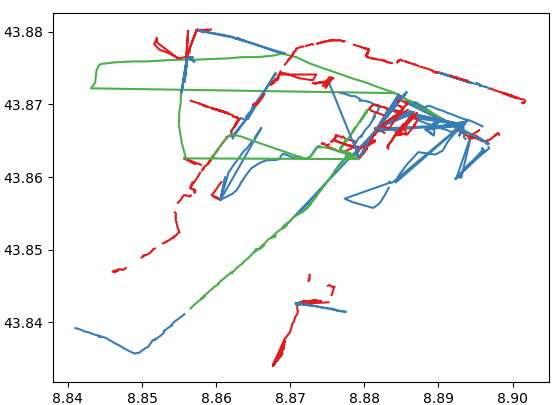
\includegraphics[width=\columnwidth]{spreaddelta-result}
		\caption{Spreaddelta heuristic line plot}
		\label{fig:spreaddelta-result}
	\end{figure}
	
	\item \textit{edgedelta heuristic}: in figure \ref{fig:edgedelta-result} you can see how the trajectories are clusterized in relation to the start and end positions of each trajectory generated by \textit{timedelta heuristic}. This heuristic performs some good results, because it is able to recognize the neighbours trajectories, but there are also some result not expected due to the problem of bimodal distribution.  
	
	\begin{figure}[bt]
		\centering
		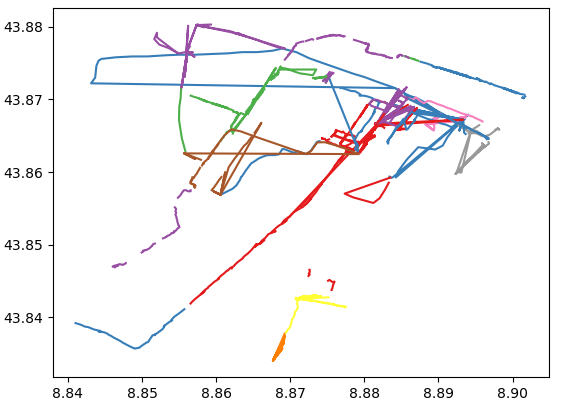
\includegraphics[width=\columnwidth]{edgedelta-result}
		\caption{Edgedelta heuristic line plot}
		\label{fig:edgedelta-result}
	\end{figure}
	
	\item \textit{coorddelta heuristic}: in figure \ref{fig:coorddelta-result} you can see the trajectories clusterized with both \textit{edgedelta} and \textit{spreaddelta} techniques. It shows the same issues of \textit{edgedelta heuristic}, but, with the \textit{spreaddelta heuristic} addition, the trajectories are even more selective, to the point of returning nearly to the initial trajectories. This heuristic can be useful only if you want a model that slightly clusterize the trajectories.
	
	\begin{figure}[bt]
		\centering
		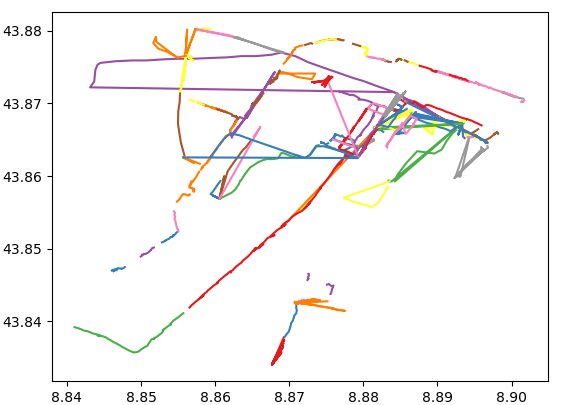
\includegraphics[width=\columnwidth]{coorddelta-result}
		\caption{Coorddelta heuristic line plot}
		\label{fig:coorddelta-result}
	\end{figure}

\end{itemize}

For clustering algorithms, in addition to graph analysis, I also use the \textit{Silhouette} validation. To evaluate the number of clusters for the algorithms that need it as parameter, I executed \textit{K-Means} for a number of cluster in a range from 1 to 30 and I calculated for each cluster number the \textit{WCSS error}. Then I plot the \textit{WCSS} graph and I used \textit{Elbow method} to choose the best value to use. As result of \textit{WCSS} graph, I chose to set 5 clusters. 

\begin{figure}[bt]
	\centering
	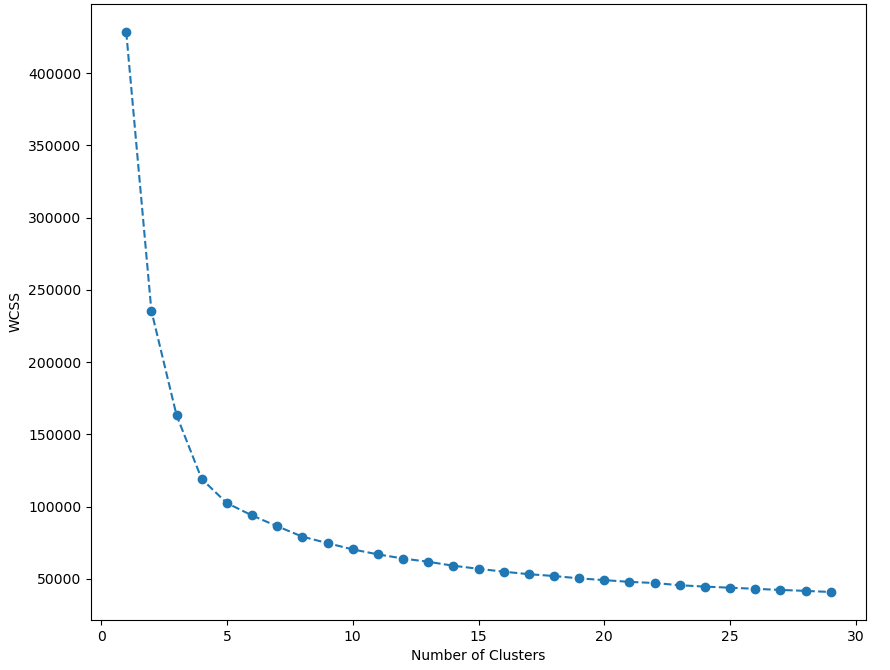
\includegraphics[width=\columnwidth]{wcss}
	\caption{Within Cluster Sum of Squares (WCSS) graph for Elbow method in range 1 to 30 with K-Means}
	\label{fig:wcss}
\end{figure}

The results of clustering techniques are the following: 

\begin{itemize}
	\item \textit{Gaussian Mixture}: performs bad result \ref{fig:gaussian-mixture-line} and the silhouette validation confirms it.
	
	\begin{figure}[bt]
		\centering
		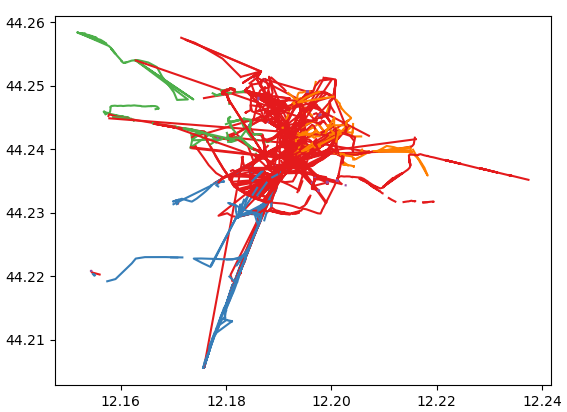
\includegraphics[width=\columnwidth]{gaussian-mixture-plot}
		\caption{Gaussian Mixture line plot with silhouette -0.02}
		\label{fig:gaussian-mixture-line}
	\end{figure}

	\item \textit{Mean Shift}: obtains the best result in terms of silhouette validation. The number of cluster generated is only 3 because \textit{Mean Shift}, at the end of algorithm, performs a pruning operation of similar centres, taking only the more significant. In general, for trajectory clustering, I would like to obtain more clusters, but this is also an alert that the number of clusters can't be really higher. 
	
	\begin{figure}[bt]
		\centering
		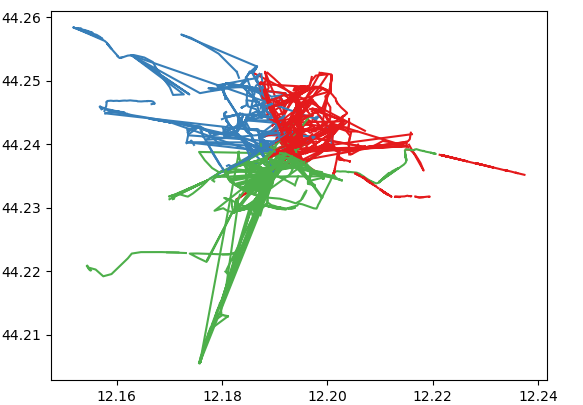
\includegraphics[width=\columnwidth]{mean-shift-plot}
		\caption{Mean Shift line plot with silhouette 0.40}
		\label{fig:mean-shift-line}
	\end{figure}

	\item \textit{Full Hierarchical Agglomerative}: worst both in silhouette validation term and representation term \ref{fig:full-agglomerative-line}, but the main issue of this technique is a huge memory cost. The dedrogram of this hierarchical algorithm is shown in the this figure \ref{fig:full-agglomerative-dendrogram}. 
	
	\begin{figure}[bt]
		\centering
		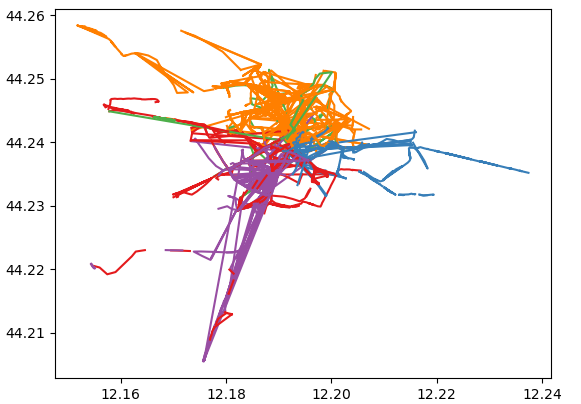
\includegraphics[width=\columnwidth]{full-agglomerative-plot}
		\caption{Full Hierarchical Agglomerative line plot with silhouette 0.16}
		\label{fig:full-agglomerative-line}
	\end{figure}

	\begin{figure}[bt]
		\centering
		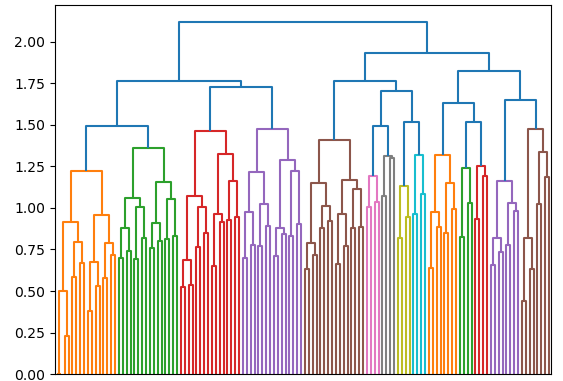
\includegraphics[width=\columnwidth]{full-agglomerative-dendrogram}
		\caption{Full Hierarchical Agglomerative dendrogram up to level 5 of merge}
		\label{fig:full-agglomerative-dendrogram}
	\end{figure}

	\item \textit{Ward Hierarchical Agglomerative}: performs well because it tries to group the centre of the city. It is really similar to \textit{K-Means}, it is not as accurate as \textit{K-Means}, but the main problem, like the \textit{Full} version of this technique, is the huge memory cost. The dedrogram of this hierarchical algorithm is shown in the this figure \ref{fig:ward-agglomerative-dendrogram}. 
	
	\begin{figure}[bt]
		\centering
		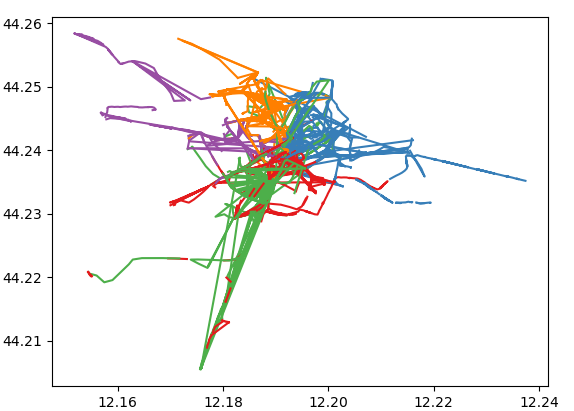
\includegraphics[width=\columnwidth]{ward-agglomerative-plot}
		\caption{Ward Hierarchical Agglomerative line plot with silhouette 0.28}
		\label{fig:ward-agglomerative-line}
	\end{figure}
	
	\begin{figure}[bt]
		\centering
		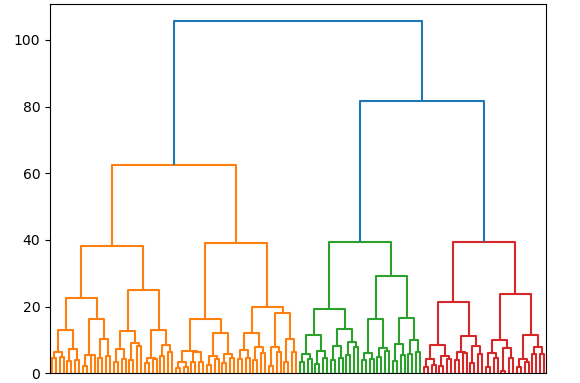
\includegraphics[width=\columnwidth]{ward-agglomerative-dendrogram}
		\caption{Ward Hierarchical Agglomerative dendrogram up to level 5 of merge}
		\label{fig:ward-agglomerative-dendrogram}
	\end{figure}

	\item \textit{K-Means}: it is the simplest algorithm but maybe the one that produces the best results. Even if it uses a distance metric to calculate the clusters, it performs very well not only in terms of plot representation, but also in silhouette value. In addition, it is really fast and cheap in memory. The main problem of this clustering result is the mixture of clusters in the city centre, that creates uncertainty.
	
	\begin{figure}[bt]
		\centering
		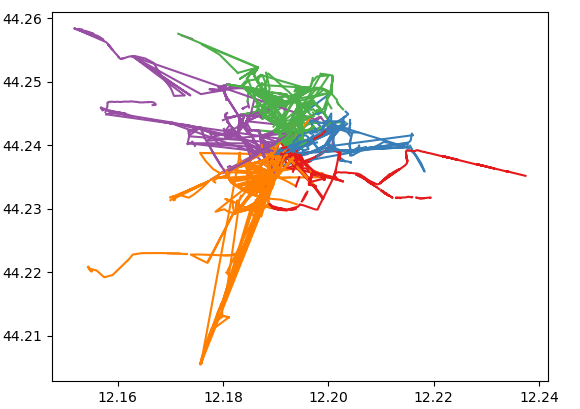
\includegraphics[width=\columnwidth]{k-means-plot}
		\caption{K-Means line plot with silhouette 0.352}
		\label{fig:k-means-line}
	\end{figure}
	
\end{itemize}

% CONCLUSION
\section{Conclusion}
The best result are the one performed by \textit{K-Means}: the feature are extracted with \textit{Standardization}, \textit{Normalization} and \textit{PCA} with my custom feature subset implementation, the number of cluster given as input is estimated through the \textit{Elbow method} from \textit{WCSS} graph, and the results are given in terms of plot representation and \textit{Silhouette score}. 

In particular the feature extraction phase has been performed with different features configuration. The best result is produced with my custom implementation of PCA on the following subset of features: 

\begin{align}
\{ &\{ latitude\} , \{longitude\}, \notag\\
 &\{spread\-latitude, spread\-longitude\}, \notag\\
 &\{edge\-latitude\-start, edge\-latitude\-stop, \notag\\ 
 &\phantom{\{}edge\-longitude\-start, edge\-longitude\-stop\} \}\notag
\end{align} 

but it doesn't perform result widely better than the traditional PCA approach based on the $80\%$ of cumulative variance. 

Moreover, feature extraction without time features produces better clustering result. Time is a feature dimension that brings cluster algorithms to a worse prediction, because the same trajectory could be travelled in different time and instead I want to find the common trajectory independently by time. On the other hand, time is very useful to find subgroups of the same trajectory, as performed by \textit{timedelta heuristic}.

Furthermore, I tried to compare \textit{K-Means} clustering with and without PCA. The figure \ref{fig:kmeans-without-pca} shows \textit{K-Means} clustering algorithm performed without PCA on latitude and longitude features only. This comparison shows how PCA improve the variance on clustering prediction, and the presence of heuristic features maintains the rental division, on which the heuristic algorithms has been executed.  

\begin{figure}[bt]
	\centering
	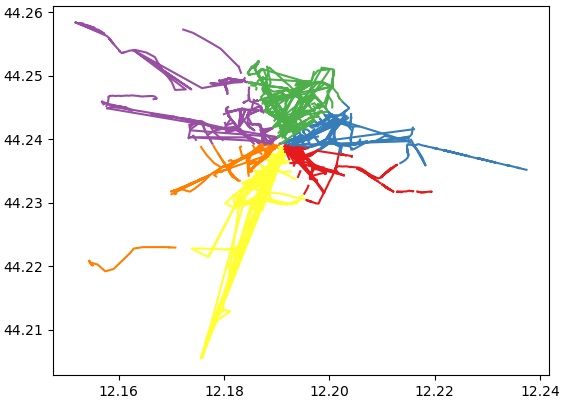
\includegraphics[width=\columnwidth]{kmeans-without-pca}
	\caption{K-Means without PCA with only latitude and longitude features}
	\label{fig:kmeans-without-pca}
\end{figure}

The tests performed shows also how difficult is the clustering operation on trajectories very distant from each other. In fact, the positions of this dataset involves mainly two Italy cities and a clustering algorithm on both will try to create 2 clusters. Since I would like to obtain more cluster and to group trajectory inside the cities, I tried to increment the number of clusters. A \textit{K-Means} clustering execution on the whole positions with 5 clusters performs really bad results (figure \ref{fig:kmeans-bad}). Therefore, clustering has always to be performed on a specific region of interest in order to optimize the results. This is the reason why clustering techniques has been performed on each city individually.

\begin{figure}[bt]
	\centering
	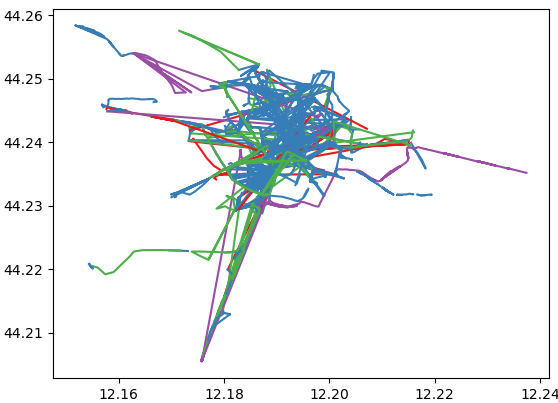
\includegraphics[width=\columnwidth]{kmeans-bad}
	\caption{K-Means with 5 clusters, PCA, Standardization and Normalization performed on all positions showed on one city}
	\label{fig:kmeans-bad}
\end{figure}

Lastly, I noticed that \textit{silhouette score} is never higher than $0.5$, while its maximum value could arrive to $1.0$. This score could indicate that the result is not very good, but actually \textit{silhouette score} is not an validation methodology so reliable, because it depends a lot on the data you are dealing with. In particular, \textit{silhouette validation} uses a distance metric to produce this value, therefore it will be very reliable when used for circular shape clustering (in 2D) but for other type of distribution, you shouldn't give it too much importance, but rather consider a visual representation of results. In our case, trajectories will hardly have a circular shape, consequently an average positive silhouette score of $0.3$ is pretty good for this kind of clustering.

For sure, \textit{edgedelta} and \textit{coorddelta} heuristic can be improved, and more advanced clustering techniques can be implemented in order to obtain better results. 

%\begin{figure*}[bt]
%	\centering
%	\includegraphics[width=\textwidth]{efsmM}
%	\caption{EFSM Moltiplicatore Floating-Point}
%	\label{fig:efsmM}
%\end{figure*}

\bibliographystyle{IEEEtran}
\bibliography{biblio}

\begin{figure*}
	\centering
	\caption{Original dataset ER model}
	\label{original-dataset-diagram}
	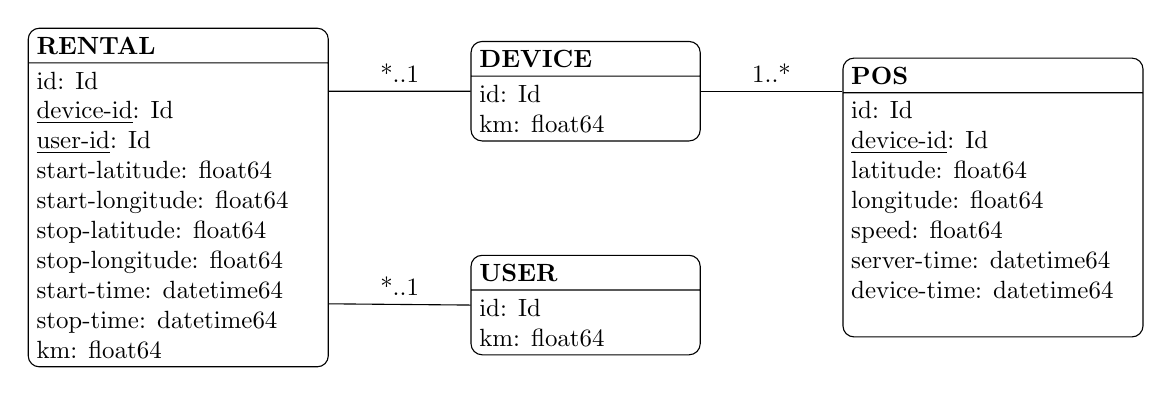
\begin{tikzpicture}[node distance=2cm, scale=0.9, transform shape]
	\node (rental) [rectangle, draw=black, rounded corners, text justified, text width=4cm, rectangle split, rectangle split parts=2]
	{
		\textbf{RENTAL}
		\nodepart{second}
		id: Id\\
		\underline{device-id}: Id\\
		\underline{user-id}: Id\\
		start-latitude: float64\\
		start-longitude: float64\\
		stop-latitude: float64\\
		stop-longitude: float64\\
		start-time: datetime64\\
		stop-time: datetime64\\
		km: float64
	};
	\node (device) [rectangle, draw=black, rounded corners, text justified, text width=3cm, rectangle split, rectangle split parts=2, right=of rental, yshift=1.5cm]
	{
		\textbf{DEVICE}
		\nodepart{second}
		id: Id\\
		km: float64
	};
	\node (pos) [rectangle, draw=black, rounded corners, text justified, text width=4cm, rectangle split, rectangle split parts=2, right=of device, yshift=-1.5cm]
	{
		\textbf{POS}
		\nodepart{second}
		id: Id\\
		\underline{device-id}: Id\\
		latitude: float64\\
		longitude: float64\\
		speed: float64\\
		server-time: datetime64\\
		device-time: datetime64\\
	};
	\node (user) [rectangle, draw=black, rounded corners, text justified, text width=3cm, rectangle split, rectangle split parts=2, below=of device, yshift=0.4cm]
	{
		\textbf{USER}
		\nodepart{second}
		id: Id\\
		km: float64
	};

	\draw ([yshift=1.5cm]rental.east) -- node[above]{*..1}  (device.west);
	\draw ([yshift=-1.5cm]rental.east) -- node[above]{*..1} (user.west);
	\draw (device.east) -- node[above]{1..*} ([yshift=1.5cm]pos.west);
	\end{tikzpicture}
\end{figure*}

\begin{figure*}
	\centering
	\caption{Generated dataset ER model}
	\label{generated-dataset-diagram}
	\begin{tikzpicture}[node distance=2cm, scale=0.9, transform shape]
	\node (rental) [rectangle, draw=black, rounded corners, text justified, text width=4cm, rectangle split, rectangle split parts=2]
	{
		\textbf{RENTAL}
		\nodepart{second}
		id: Id\\
		\underline{device-id}: Id\\
		\underline{user-id}: Id\\
		start-latitude: float64\\
		start-longitude: float64\\
		stop-latitude: float64\\
		stop-longitude: float64\\
		start-time: datetime64\\
		stop-time: datetime64\\
		km: float64
	};
	\node (pos) [rectangle, draw=black, rounded corners, text justified, text width=9cm, rectangle split, rectangle split parts=2, right=of rental]
	{
		\textbf{POS}
		\nodepart{second}\begin{multicols*}{2}
		id: Id\\
		\underline{rental-id}: Id\\
		timedelta-id: Id\\
		spreaddelta-id: Id\\
		edgedelta-id: Id\\
		coorddelta-id: Id\\
		latitude: float64\\
		longitude: float64\\
		spread-latitude: float64\\
		spread-longitude: float64\\
		\vfill
		\columnbreak
		edge-latitude-start: float64\\
		edge-latitude-stop: float64\\
		edge-longitude-start: float64\\
		edge-longitude-stop: float64\\
		speed: float64\\
		server-time: datetime64\\
		device-time: datetime64\\
		time-gap: float64\\
		\end{multicols*}
	};
	\node (device) [rectangle, draw=black, rounded corners, text justified, text width=3cm, rectangle split, rectangle split parts=2, left=of rental, yshift=1.5cm]
	{
		\textbf{DEVICE}
		\nodepart{second}
		id: Id\\
		km: float64
	};
	\node (user) [rectangle, draw=black, rounded corners, text justified, text width=3cm, rectangle split, rectangle split parts=2, left=of rental, yshift=-1.5cm]
	{
		\textbf{USER}
		\nodepart{second}
		id: Id\\
		km: float64
	};
	
	\draw ([yshift=1.5cm]rental.west) -- node[above]{1..1}  (device.east);
	\draw ([yshift=-1.5cm]rental.west) -- node[above]{ 1..*} (user.east);
	\draw (rental.east) -- node[above]{1..*} (pos.west);
	\end{tikzpicture}
\end{figure*}

\end{document}
